\section{Fuentes de ruido inteligentes serie N4000A}
	\subsection{Descripción general}
	
	Para realizar mediciones de figura de ruido con el sistema de la figura \ref{Fig:BancoPruebasFuenteRuido}, se requiere de un generador de señal de ruido para excitar al dispositivo en su entrada y obtener como repuesta los parámetros de ruido. Por ser una señal de naturaleza aleatoria, sus característica no pueden ser dadas de forma determinista (en función del tiempo), sino que se especifican en términos estadísticos (valores de rms) y en función de espectro de su  densidad de potencia. El nivel de exactitud y precisión con el cual se conozcan estos valores determinan el nivel de exactitud y precisión de las mediciones de parámetros de ruido: no podrán ser mejores que los de la fuente.  
	
	\begin{figure}[h!]
		\centering
		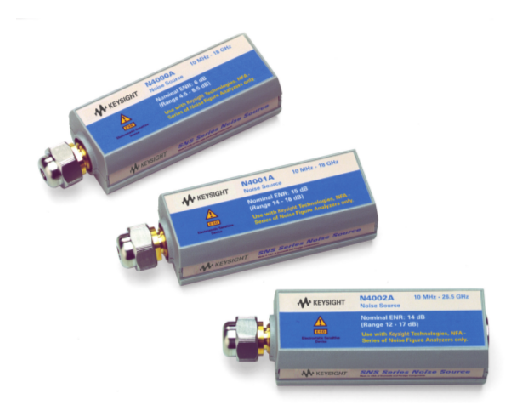
\includegraphics[width=8cm]{Imagenes/FuenteRuidoSNS.png}
		\caption{Fuente de ruido inteligente (SNS) de la serie N4000}
		\label{Fig:FuenteRuidoSNS}
	\end{figure}
	
	Las fuentes de ruido empleadas en su sistemas de calibración requieren de una fuente de ruido que entregue una señal con características plenamente conocidas, estandarizadas, estables. En el sistema de la figura \ref{Fig:BancoPruebasFuenteRuido} pueden emplearse dos series de modelos de fuentes de ruido, los modelos de la serie 346 y las fuentes de ruido inteligentes de la serie N4000, como se aprecia en la figura \ref{Fig:ModelosFuenteRuido}. Éstas últimas son las fuentes de ruido con las que cuenta el CENDIT.
	
	\begin{figure}[h!]
		\centering
		\includegraphics[width=15cm]{Imagenes/FuentesRuido.png}
		\caption{Modelos para fuentes de ruido series 346 y N4000}
		\label{Fig:ModelosFuenteRuido}
	\end{figure}
	
	\subsection{Modo de operación}
	Las fuentes de ruido de la serie N4000 emplean un diodo semiconductor de silicio con polarización inversa como elemento generador de ruido de banda ancha. El nivel de potencia de ruido a la salida de la fuente es una función de la corriente inversa de polarización en el diodo. Las fuentes de ruido de la serie N4000 generan una señal de ruido con dos niveles de potencia distintos, conocidos como el \emph{nivel encendido (ON)} y el \emph{nivel apagado (OFF)}. 
	
	El nivel OFF ocurre cuando se elimina la corriente de inversa en el diodo, la fuente genera ruido debido a la agitación térmica de sus componentes internos con un nivel de potencia acorde a la temperatura física de la fuente. Se modela matemáticamente como ruido térmico de banda ancha, proporcional a la resistencia de salida de la fuente de ruido y la temperatura física de la misma. 
	
	El nivel ON sucede cuando se aplica la corriente de polarización inversa al diodo, el ruido a la salida se incrementa de manera sustancial. En este estado, la fuente aún genera el ruido térmico pero agrega una componente adicional de ruido, conocida como ruido en exceso. El ruido en exceso no es de naturaleza térmica, no depende de la temperatura física de la fuente, pero puede modelarse matemáticamente como tal por medio de la temperatura equivalente de la fuente de ruido.
	
	Las características de salida para una fuente de ruido vienen dadas en función de su rango de frecuencia y el nivel de potencia de ruido que entregan a su salida, expresada por la razón de ruido en exceso (ENR). Las fuentes de ruido de la serie N4000 poseen valores de nominales de ENR en el rango de 6 a 15 \si{\dB} para frecuencias entre 10 \si{\mega\hertz} y 26.6 \si{\giga\hertz}, tal como se indica en la tabla \ref{Tab:RangosFuentesRuido}.
	
	Los valores de ENR son calibrados en puntos específicos de frecuencia.
	
	\begin{table}[h!]
		\centering
		\begin{tabular}{cccc}
			\toprule
			Modelo de NS	&	ENR nominal (\si{\decibel})	& Rango de ENR (\si{\decibel})	&	Rango de frecuencia			\\
			\midrule	
			N4000A 	&	6.0	&	4.5 - 6.5	&	10 \si{\mega\hertz} - 18 \si{\giga\hertz} \\
			\midrule				
			N4001A 	&	15.0	&	14 - 16	&	10 \si{\mega\hertz} - 18 \si{\giga\hertz} \\
			\midrule	
			N4002A 	&	16.0	&	12 - 17	&	10 \si{\mega\hertz} - 26.5 \si{\giga\hertz} \\
			\bottomrule			
		\end{tabular}
		\caption{Rangos de ENR nominal para fuentes de ruido serie N4000}
		\label{Tab:RangosFuentesRuido}
	\end{table}
	
	Se emplean fuentes de ruido con bajo valor de ENR para minimizar el error por la no linealidad del detector de ruido. El error sera menor si la medida se realiza sobre un rango menor, en la zona de mayor linealidad, del detector de ruido. En este caso se emplea una fuente con ENR de 6 dB. [3]
	
	Estos dos niveles de ruido, ON y OFF, se usan para medición de ganancia y ruido agregado por parte del dispositivo bajo prueba, y por consiguiente, su figura de ruido.	
	
	\subsection{Estructura interna}
			
	En la figura \ref{Fig:DiagramaBloquesFuenteRuido} se muestra un diagrama de bloques que muestra la estructura interna de las fuentes de ruido de la serie N4000. La fuente de ruido requiere de una tensión de alimentación de +28 \si{\volt} para su operación. En las fuentes de ruido N4000A y N4001A, un inversor de voltaje interno convierte esta tensión a -25 \si{\volt} y la aplica al regulador de corriente que alimenta al bloque regulador de corriente para alimentar al diodo generador de ruido. El modelo N4002 emplea una polarización positiva, así que no posee un inversor de voltaje en su interior.
	
	El bloque regulador de corriente se encarga además de realizar la conmutación necesaria para producir los estados de ruido ON y OFF. Cuando se polariza el diodo de forma inversa, éste produce ruido de banda ancha el cual se inyecta al atenuador. El atenuador fija el valor final de ENR y establece la impedancia de salida de la SNS. Este atenuador es de 16 dB en los modelos N4000A para entregar a  su salida un ENR de 5 dB. Los modelos de SNS N4001A y N4002A utilizan un atenuador de 6 dB para entregar un valor nominal de ENR de 15 dB.		

	Los valores de ENR son dados en puntos de frecuencia cardinales sobre el rango de frecuencia de cada fuente, las parejas de datos frecuencia/ENR están almacenado en una EEPROM interna así como también los datos de incertidumbre y el coeficiente de reflexión complejo en ambos estados ON y OFF, documentados en el reporte de calibración. [1.8]. El ENR relaciona el nivel de ruido en exceso al ruido obtenido con la temperatura estándar de 296 K o al nivel de ruido que existe a la temperatura a estándar de 296 K. El valor de ENR no incluye la componente de ruido en OFF. 
	
	Las fuentes de ruido SNS poseen en su interior memoria EEPROM no volátil, en esta memoria residen los datos que caracterizan a una fuente de ruido particular en función de la frecuencia, como lo son el ENR y el coeficiente de reflexión, además de que incluyen modelo, numero de serial y la configuración de la intensidad de corriente de diodo y datos de calibración. Estos datos son almacenados  durante la calibración en fabrica de cada NS. Se encuentran dentro de un archivo en formato de texto plano, el incluye una tabla con filas de valores valores para ENR, coeficiente de reflexión con sus respectivas incertidumbres para puntos cardinales de frecuencia, distribuidos de manera uniforme sobre el rango de operación de la fuente de ruido. 	

	El NFA puede descargar los datos de ENR y coeficiente de reflexión, leerlos y modificarlos, para emplearlos en los cálculos de figura de ruido. Es por esta razón que esta fuentes se conocen como "inteligentes".	
	
	Las NS de la serie N4000 cuentan con un termómetro digital, se encuentra térmicamente acoplado al ensamble de microondas y le permita registrar la temperatura ambiente. EL NFA puede leer el valor de temperatura ambiente de este termómetro, lo emplea en los cálculos de figura de ruido en donde se necesite el valor de la temperatura fria, 			

	
	\begin{figure}[h!]{18}
		\centering
		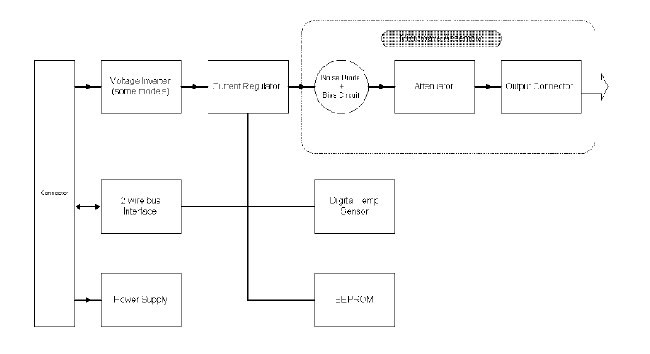
\includegraphics{Imagenes/DiagramaBloquesFuenteRuido.png}
		\caption{Diagrama de bloques para una fuente de ruido serie N4000}
		\label{Fig:DiagramaBloquesFuenteRuido}
	\end{figure}
	

	\subsection{Interfaces}
	Las fuentes de ruido inteligentes disponen de dos interfaces de tipo eléctrico: un interfaz de señal de RF y {\textmu}F y otra interfaz para comunicación de datos. 
	
	\subsubsection{Interfaz eléctrica: señal de ruido}
	Las características de las fuentes de ruido se determinan por tres parámetros. El más importante de estos es su \emph{razón de ruido excedente (ENR)}, la cual indica, de forma indirecta, la potencia de ruido nominal que la fuente puede entregar. Viene dada por una razón de potencias de ruido o de temperaturas de ruido equivalentes, es una cantidad adimensional, pero es practica común expresarla en decibelios. En la tabla \ref{Tab:RangosNominalesENR} se indican los niveles nominales para las fuentes de ruido de las series 346 y N4000.
	
	\begin{table}[h!]
		\centering
		\begin{tabular}{cc}
			\toprule
			Modelo de NS	&	Rango de ENR (\SI{}{\decibel})		\\
			\midrule	
			N4000A / 346A	&	4.5 - 6.5 					\\
			\midrule				
			N4001A / 346B	&	14 - 16  					\\
			\midrule	
			N4002A / 346C	& 	12 - 17 					\\
			\bottomrule			
		\end{tabular}
		\caption{Rangos de ENR nominal para fuentes de ruido}
		\label{Tab:RangosNominalesENR}
	\end{table}

	Los dos parámetros restantes que describen una fuente de ruido están relacionados con el acople con el resto del sistema, estos son el ROE (SWR) y su coeficiente de reflexión. Los tres parámetros descriptivos, el ENR, la ROE y el coeficiente de reflexión son dependientes de la frecuencia. En la tabla \ref{Tab:CaracteristicasElectricasN4000} se resumen estos datos para las fuentes de ruido de la serie N4000 para los rangos de frecuencia respectivos a cada modelo de fuente de ruido.
	
	\begin{table}[h!]
		\centering
		\begin{tabular}{cccc}
				\toprule
					& Rango de frecuencia & ROE máxima & Coeficiente de reflexión 	\\
					& (\si{\giga\hertz})  &			   & para los estados ON / OFF	\\
				\midrule
			N4000A	&	0.01 - 1.5	&	< 1.06 : 1	&	0.03	\\
					&	1.5	- 3.0	&	< 1.06 : 1	&	0.03 	\\
					&	3.0 - 7.0	&	< 1.13 : 1	&	0.06	\\
					&	7.0	- 18.0	&	< 1.22 : 1	&	0.10	\\
				\midrule
			N4001A	&	0.01 - 1.5	& 	< 1.15 : 1 	&	0.07	\\
					&	1.5 - 3.0	&	< 1.15 : 1	& 	0.07	\\
					& 	3.0 - 7.0	& 	< 1.20 : 1	&	0.09	\\
					&	7.0	- 18.0	&	< 1.25 : 1	&	0.11	\\
				\midrule
			N4002A	&	0.01 - 1.5	&	< 1.22 : 1	& 	0.10	\\
					&	1.5	- 3.0	&	< 1.22 : 1	&	0.10	\\
					&	7.0	- 18.0	&	< 1.25 : 1	&	0.11	\\
					&	18.0 - 26.5	&	< 1.35 : 1	&	0.15	\\
				\bottomrule			
		\end{tabular}
		\caption{Características eléctricas para fuentes de ruidos SNS serie N4000}
		\label{Tab:CaracteristicasElectricasN4000}
	\end{table}
	
	\begin{table}[h!]
		\centering
		\begin{tabular}{cccc}
			\toprule
			Modelo de SNS		&	N4000A		&	N4001A		&	N4002A	\\
			\midrule
			Rango de frecuencia	&	\SI{10}{\mega\hertz} a \SI{18}{\giga\hertz} & \SI{10}{\mega\hertz} - \SI{18}{\giga\hertz} & \SI{10}{\mega\hertz} - \SI{18}{\giga\hertz} \\
			\midrule
			Conector			&	\multicolumn{3}{c}{APC \SI{3.5}{\milli\meter} con opción de Tipo-M (m)}	\\
			\midrule
			ENR nominal	(\si{\decibel})		&	6 		&	6		&	30		\\
			\midrule
			Rango de ENR (\si{\decibel}) 	& 4.5 - 6.5 & 14 - 16	& 12 - 17 	\\
			\midrule
			Rango de F en el DUT (\si{\decibel}) & < 20		& < 30 		& 	?	 \\
			\midrule
			Rango de temperatura (\si{\degreeCelsius}) 	& \multicolumn{3}{c}{0 a 55} \\
			\midrule
			Precisión 				& \multicolumn{3}{c}{$\pm 1 a \SI{25}{\degreeCelsius}$} \\
									& \multicolumn{3}{c}{$\pm 2 de 0 a \SI{55}{\degreeCelsius}$} \\
			\midrule
			Impedancia (\si{\ohm})  & \multicolumn{3}{c}{ 50 } \\
			\midrule
			Máxima potencia inversa (\si{\watt}) 	& \multicolumn{3}{c}{1} \\
			\midrule
			Variación de ENR con temperatura 		& \multicolumn{3}{c}{ < \SI{0.01}{\decibel} / \si{\degreeCelsius} de \SI{30}{\mega\hertz} a \SI{26}{\giga\hertz}} \\
			\midrule
			Sensor de temperatura 	& Rango 		& \multicolumn{2}{c}{0 a \SI{55}{\degreeCelsius}} \\
									& Resolución 	& \multicolumn{2}{c}{\SI{0.25}{\degreeCelsius}} \\
									& Precisión 	& \multicolumn{2}{c}{$\pm \SI{1}{\degreeCelsius} a \SI{25}{\degreeCelsius}$} \\
									&				& \multicolumn{2}{c}{$\pm \SI{2}{\degreeCelsius} de 0 a \SI{55}{\degreeCelsius}$} \\ 
			\bottomrule									
		\end{tabular}
	\end{table}	
	


	Los valores de ENR son dados en puntos de frecuencia cardinales sobre el rango de frecuencia de cada fuente, las parejas de datos frecuencia/ENR están almacenado en una EEPROM interna así como también los datos de incertidumbre y el coeficiente de reflexión complejo en ambos estados ON y OFF, \ documentados en el reporte de calibración. [1.8]. El ENR relaciona el nivel de ruido en exceso al ruido obtenido con la temperatura estándar de 296 K o al nivel de ruido que existe a la temperatura a estándar de 296 K. El valor de ENR no incluye la componente de ruido en OFF. 
	
	\subsubsection{Interfaz de comunicaciones}
	Las fuentes de ruido almacenan los datos de calibración en su memoria EEPROM interna y poseen un termómetro digital, el NFA N8975 cuenta con la capacidad para descargar estos datos de calibración y leer el valor de temperatura, para luego emplearlos en los cálculos de figura de ruido.
	
	La transferencia de datos entre la fuente de ruido y el NFA se realiza a través de un bus serial (two-wire bus). 
	
	El NFA debe proveer una alimentación de +5 V a la interfaz serial, la memoria EEPROM y el sensor digital de temperatura. Las fuentes de ruido SNS utiliza emplean un bus serial (two-wire bus) para transferencia de datos entre la fuente de ruido y el NFA. 
	
	\subsection{Selección de fuente de ruido}
	Se emplean fuentes de ruido con bajo valor de ENR para minimizar el error por la no linealidad del detector de ruido. El error sera menor si la medida se realiza sobre un rango menor, en la zona de mayor linealidad, del detector de ruido. En este caso se emplea una fuente con ENR de 6 dB.
	
	Se debe emplear una fuente de ruido con un conector adecuado para el DUT en vez de emplear un adaptador, en especial para dispositivos de alta ganancia. Los valores de ENR para una fuente de ruido aplican solo hasta el su conector. Un adaptador añade perdidas a los valores de ENR, la incertidumbre en estas perdidas incrementa la  total en la medición. Si se usa un adaptado, se deben tomar en cuenta sus perdidas. [3].
	
	Es importante emplear un NS con el menor cambio en su impedancia de salida entre sus estado de encendido y apagado. Estos cambios de impedancia alteran el acoplamiento entre la NS y el DUT lo que conlleva a cambos en la ganancia y en la figura de ruido del DUT. Las fuentes de ruido comerciales de 6dB ENR limitan el cambio del coeficiente de reflexión entre los estados ON y OFF a menos de 0.01 a frecuencias hasta de 18 GHz. [3]
	
	Las fuentes de ruido con bajo valor de ENR son ideales para medición, sin embargo, las fuentes de alto ruido son necesarias para calibrar el rango dinámico completo del instrumento. Los NFA pueden tomar en cuenta las distintas tablas de ENR requeridas para la calibración y medida. [3]
	
	Una fuente con un bajo valor de ENR necesitara en el instrumento un menor valor de atenuación para cubrir el rango dinámico, excepto cuando la ganancia del DUT es muy alta. Emplear menor atenuación redice la figura de ruido del instrumento de medición, lo cual a su vez reduce la incertidumbre en la medición. [3]	
	